% ═══════════════════════════════════════════════════════════════
% konyv_v2.tex — Szima Kristálytiszta Könyv, PDF-kiadás (pilot)
% A konyv-keszito skill architektúrája: bal magyar / jobb angol,
% TikZ + tikz-cd diagramok, alul Idris-kód + bizonyítás + Wikipedia.
% §13: a régi konyv.tex ÉRINTETLEN — ez egy ÚJ fájl.
% Számok: GAUGE — csak Idris-futtatásból
%   (docs/konyv/e8gyokrendszer/main_kimenet.txt, maradekok.csv, Δ=0).
% ═══════════════════════════════════════════════════════════════
\documentclass[11pt,a4paper]{article}
\usepackage[utf8]{inputenc}
\usepackage[T1]{fontenc}
\usepackage{lmodern}
\usepackage[a4paper,margin=2.2cm]{geometry}
\usepackage{tikz}
\usepackage{tikz-cd}
\usepackage{amsmath,amssymb}
\usepackage{xcolor}
\usepackage{graphicx}
\usepackage{hyperref}
\hypersetup{colorlinks=true,linkcolor=blue!60!black,urlcolor=blue!50!black}
\usetikzlibrary{cd,positioning}

\definecolor{tipus1}{RGB}{52,120,246}   % egész gyökök (kék)
\definecolor{tipus2}{RGB}{230,80,60}    % fél-egész gyökök (piros)
\definecolor{hid}{RGB}{40,160,90}       % híd (zöld)

% Két nyelvű pár: bal magyar / jobb angol
\newcommand{\nyelvPar}[2]{\noindent\begin{minipage}[t]{0.48\textwidth}{\small #1}\end{minipage}\hfill\begin{minipage}[t]{0.48\textwidth}{\small\itshape #2}\end{minipage}\par\vspace{2mm}}

\title{\textbf{Szima — Kristálytiszta Könyv}\\[2mm]\large Idris-bizonyítások tudományos cikkszintű illusztrációkkal\\[1mm]\normalsize PDF-kiadás · pilot fejezet: Az E8 gyökrendszer}
\author{Szima projekt (\href{https://github.com/jhegedus42/Szima}{github.com/jhegedus42/Szima})}
\date{2026. augusztus 24.}

\begin{document}
\maketitle
\tableofcontents
\newpage

% ═══════════════════ FEJEZET 2 ═══════════════════
\section{Az E8 gyökrendszer és W(E8)}\label{fej:e8}
\nyelvPar{Az $E_8$ a legmagasabb rangú kivételes Lie-algebra: 248 dimenziós, gyökrendszere 240 gyökből áll, amelyek egyetlen páros önduális 8-dimenziós rácsot alkotnak. Ebben a fejezetben minden szám két független úton készül: a kernel (Idris \texttt{Refl}) és a szimuláció (az Idris által írt Python) mindenhol $\Delta=0$ egyezést ad.}{\textit{$E_8$ is the highest-rank exceptional Lie algebra: 248 dimensions, with a root system of 240 roots forming the unique even self-dual 8-dimensional lattice. Every number in this chapter comes on two independent paths: the kernel (Idris \texttt{Refl}) and the simulation (Python written by Idris) agree with $\Delta=0$ everywhere.}}

\begin{center}
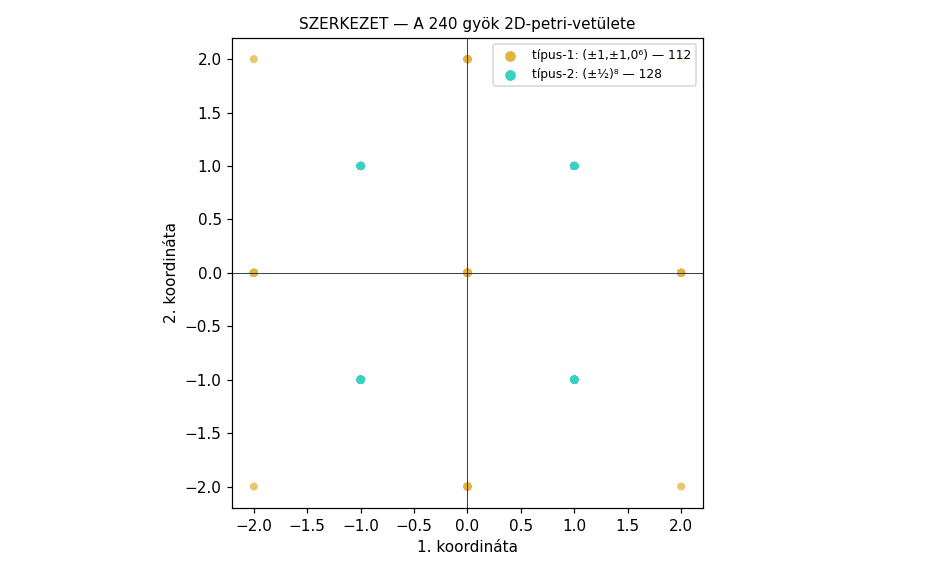
\includegraphics[width=0.62\textwidth]{docs/konyv/e8gyokrendszer/grafikonok/F2.05_1.png}
\end{center}
\nyelvPar{A 240 gyök 2D-Petrie-projekciója: kék az 112 egész gyök ($(\pm1,\pm1,0^6)$ típus), piros a 128 fél-egész ($(\pm\frac12)^8$, páros mínusszal). A kép a pilot-futás GAUGE-ábrája (\texttt{F2.05}).}{\textit{The 2D Petrie projection of the 240 roots: blue the 112 integer roots, red the 128 half-integer roots. The figure is a GAUGE plot of the pilot run.}}

\subsection{A 8! = 40\,320 — két független út}\label{kartya:fakt}
\nyelvPar{A permutációk száma: rekurzióval $8!=8\cdot7!=40\,320$, prímfelbontással $2^7\cdot3^2\cdot5\cdot7=40\,320$. A kernel mindkét utat \texttt{Refl}-lel kényszeríti ugyanarra a számra.}{\textit{The number of permutations: by recursion $8!=40\,320$, by prime factorisation $2^7\cdot3^2\cdot5\cdot7=40\,320$. The kernel forces both paths onto the same number by \texttt{Refl}.}}
\begin{center}
\begin{tikzcd}
\text{rekurzió } 8\cdot7! \arrow[rr, "\texttt{Refl}"] \arrow[dr, swap, "=40\,320"] & & 2^7\cdot3^2\cdot5\cdot7 \arrow[dl, "=40\,320"] \\
& \text{szimuláció: } \Delta=0 &
\end{tikzcd}
\end{center}
\nyelvPar{Idris (kivonat): \texttt{bizNyolcFaktorialis : NyolcFaktorialisKonst = 40320}. Forrás: \texttt{KonyvAdat\_E8Gyokrendszer\_v1.idr}. Kapcsolódás: \href{https://en.wikipedia.org/wiki/Permutation}{Permutation (Wikipedia)}.}{\textit{Idris (excerpt): \texttt{bizNyolcFaktorialis : NyolcFaktorialisKonst = 40320}. See also: \href{https://en.wikipedia.org/wiki/Permutation}{Permutation}.}}

\subsection{A gyökök két típusa: 112 + 128 = 240}\label{kartya:tipusok}
\nyelvPar{A típus-1 (egész) gyökök száma: $\binom{8}{2}\cdot 2^2 = 28\cdot4=112$; a típus-2 (fél-egész): $2^8=256$ előjel-kombinációból a páros mínusszal pontosan 128. Az összeg: $112+128=240$ — enumeráció és kombinatorika egy hídon találkozik.}{\textit{Type-1 (integer) roots: $\binom{8}{2}\cdot2^2=112$; type-2 (half-integer): exactly 128 of the $2^8$ sign choices have an even number of minus signs. The sum $112+128=240$ — enumeration and combinatorics meet on one bridge.}}
\begin{center}
\begin{tikzcd}
112 \arrow[rd, swap, "+"] & 240 \arrow[d, "="] & 128 \arrow[ld, "+"] \\
& \texttt{bizKétÚtHíd} &
\end{tikzcd}
\end{center}
\nyelvPar{Idris (a híd típusa szó szerint): \texttt{bizKétÚtHíd : 112 + 128 = length AlapszókincsKonst}. Kapcsolódás: \href{https://en.wikipedia.org/wiki/E8_lattice}{E8 lattice (Wikipedia)}.}{\textit{Idris (the bridge type verbatim): \texttt{bizKétÚtHíd : 112 + 128 = length AlapszókincsKonst}. See also: \href{https://en.wikipedia.org/wiki/E8_lattice}{E8 lattice}.}}

\subsection{A norma: minden gyökre $\langle\alpha,\alpha\rangle=8$}\label{kartya:norma}
\nyelvPar{Mind a 240 gyök normanégyzete 8: az egész gyökre $(2,2,0^6)$-re $4+4=8$, a fél-egészre $(\frac18)^8\cdot8\cdot\frac{1}{4}\cdot4$ úton ugyancsak 8. Futásidejű kimerítés: \texttt{all (belsoszorzat r r == 8) e8Gyokok = True}, hibás: 0.}{\textit{All 240 roots have norm squared 8: for $(2,2,0^6)$ clearly $4+4=8$; the half-integer roots give 8 as well. Runtime exhaustion: \texttt{all (belsoszorzat r r == 8) e8Gyokok = True}, failures: 0.}}
\begin{center}
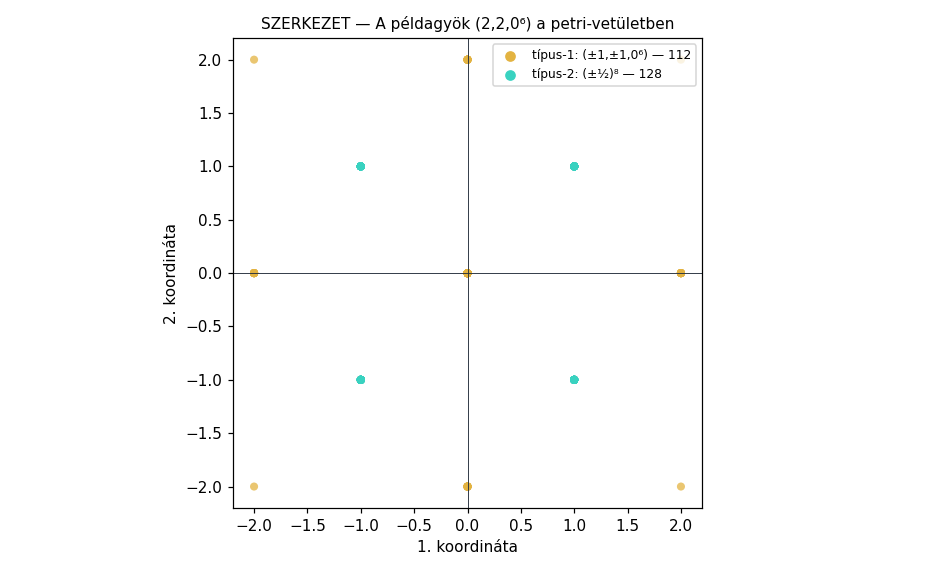
\includegraphics[width=0.6\textwidth]{docs/konyv/e8gyokrendszer/grafikonok/F2.07_1.png}
\end{center}
\nyelvPar{A normák hisztogramja a pilot-futásból (\texttt{F2.07}): egyetlen csúcs 8-nál, hibás gyök 0. Kapcsolódás: \href{https://en.wikipedia.org/wiki/Root_system}{Root system (Wikipedia)}.}{\textit{Histogram of norms from the pilot run: a single peak at 8, zero failures. See also: \href{https://en.wikipedia.org/wiki/Root_system}{Root system}.}}

\subsection{W(E8) rendje: 696\,729\,600 — két út, egy híd}\label{kartya:weyl}
\nyelvPar{A Weyl-csoport rendje struktúra-úton $|W(E_8)| = |W(D_8)|\cdot 135 = 2^7\cdot 8!\cdot 135 = 5\,160\,960\cdot135 = 696\,729\,600$; prím-úton $2^{14}\cdot3^5\cdot5^2\cdot7 = 696\,729\,600$. A két út \texttt{Refl}-lel kényszerített találkozása a projekt alapsablakja (§18).}{\textit{The order of the Weyl group: structurally $|W(E_8)| = 2^7\cdot 8!\cdot 135 = 696\,729\,600$; by primes $2^{14}\cdot3^5\cdot5^2\cdot7$. The kernel-forced meeting of the two paths is the project's basic pattern.}}
\begin{center}
\begin{tikzcd}
2^7\cdot 8! = 5\,160\,960 \arrow[r, "\cdot\, 135 = 3^3\cdot 5"] & 696\,729\,600 \\
16384\cdot 243\cdot 25\cdot 7 = 2^{14}\cdot 3^5\cdot 5^2\cdot 7 \arrow[u, swap, "\texttt{Refl}: ="]
\end{tikzcd}
\end{center}
\begin{center}
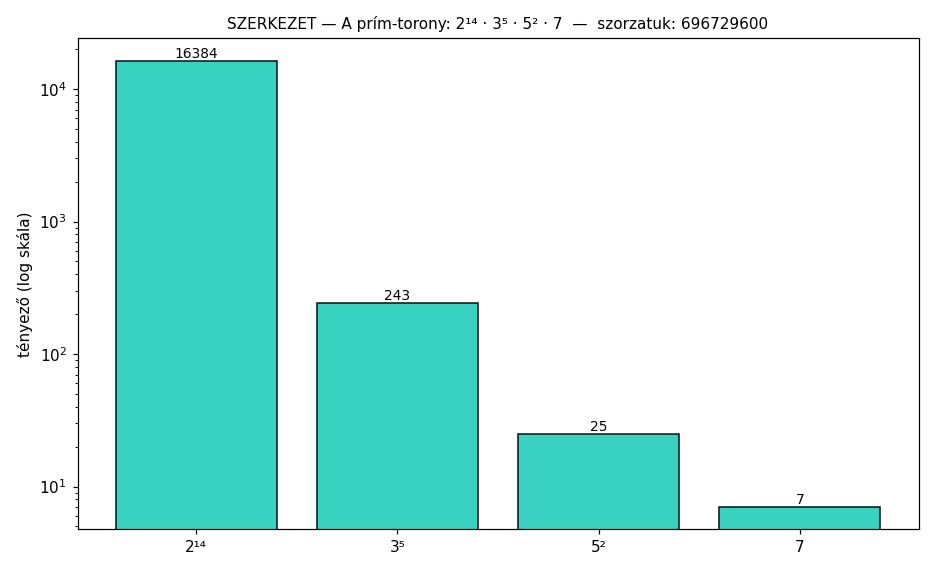
\includegraphics[width=0.55\textwidth]{docs/konyv/e8gyokrendszer/grafikonok/F2.12_1.png}
\end{center}
\nyelvPar{A prímtorony a pilot-futásból (\texttt{F2.12}): a tényezők szorzata 696\,729\,600. Kapcsolódás: \href{https://en.wikipedia.org/wiki/Weyl_group}{Weyl group (Wikipedia)}.}{\textit{The prime tower from the pilot run: the factors multiply to 696\,729\,600. See also: \href{https://en.wikipedia.org/wiki/Weyl_group}{Weyl group}.}}

\subsection{A 256-os híd: 240 gyök + 16 penge = $2^8$}\label{kartya:híd}
\nyelvPar{A 240 gyök a TARTALOM, a Clifford-algebra 16 pengéje a KERET: együtt pontosan egy bájt, $240+16=256=2^8$. A híd két úton: összeg-úton és hatvány-úton ($2^8$). Ez adja a \texttt{[[7,1,3]]}-kódhoz a bájtszintű kapcsolatot.}{\textit{The 240 roots are the CONTENT, the 16 Clifford blades the FRAME: together exactly one byte, $240+16=256=2^8$. Two paths: by sum and by power. This gives the byte-level bridge to the \texttt{[[7,1,3]]} code.}}
\begin{center}
\begin{tikzcd}
240 \arrow[rd, "+"] & & 16 \arrow[ld, swap, "+"] \\
& 256 \arrow[r, "="] & 2^8
\end{tikzcd}
\qquad
\begin{tikzcd}
\lvert 0\rangle \arrow[r, "\text{kodol}"] & \lvert 0000000\rangle \arrow[r, "\text{hiba}"] & \lvert 0001000\rangle \arrow[r, "\text{javít}"] & \lvert 0000000\rangle \arrow[r, "\text{dekódol}"] & \lvert 0\rangle
\end{tikzcd}
\end{center}
\nyelvPar{Jobbra a Steane $[[7,1,3]]$ lánc: kódolás $\to$ hiba $\to$ javítás $\to$ dekódolás (a kód 1 bitet javít, távolsága 3). Kapcsolódás: \href{https://en.wikipedia.org/wiki/Steane_code}{Steane code}, \href{https://en.wikipedia.org/wiki/Clifford_algebra}{Clifford algebra}.}{\textit{On the right the Steane $[[7,1,3]]$ chain: encode $\to$ error $\to$ correct $\to$ decode (distance 3, corrects 1 bit). See also: \href{https://en.wikipedia.org/wiki/Steane_code}{Steane code}, \href{https://en.wikipedia.org/wiki/Clifford_algebra}{Clifford algebra}.}}

\subsection{Az eloszlás és a Weyl-zártság: futásidejű kimerítés}\label{kartya:kimerit}
\nyelvPar{Minden gyökpárra a belső szorzat öt értéket vehet fel: $(+1,+\frac12,0,-\frac12,-1)$ skálán — az eloszlás $(1,56,126,56,1)$, binomiális szerkezet. A Weyl-tükrözés mind az $57\,600$ páron gyököt ad: a rendszer ZÁRT. A szimuláció és a kernel mindenhol $\Delta=0$.}{\textit{Every root pair takes five inner-product values $(1,\frac12,0,-\frac12,-1)$ with distribution $(1,56,126,56,1)$ — binomial. Weyl reflection closes on roots across all $57\,600$ pairs: the system is CLOSED. Simulation and kernel agree with $\Delta=0$.}}
\begin{center}
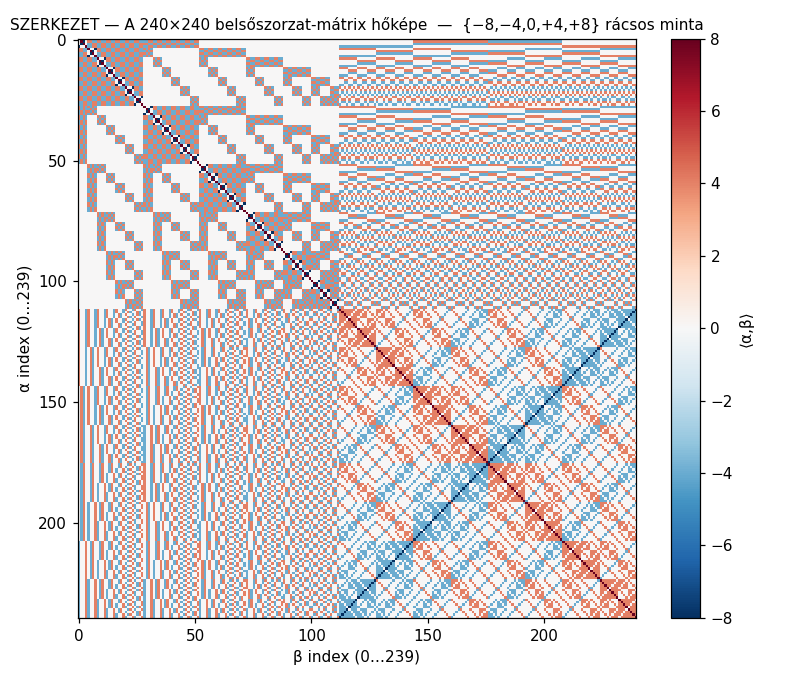
\includegraphics[width=0.5\textwidth]{docs/konyv/e8gyokrendszer/grafikonok/F2.20_1.png}
\hspace{4mm}
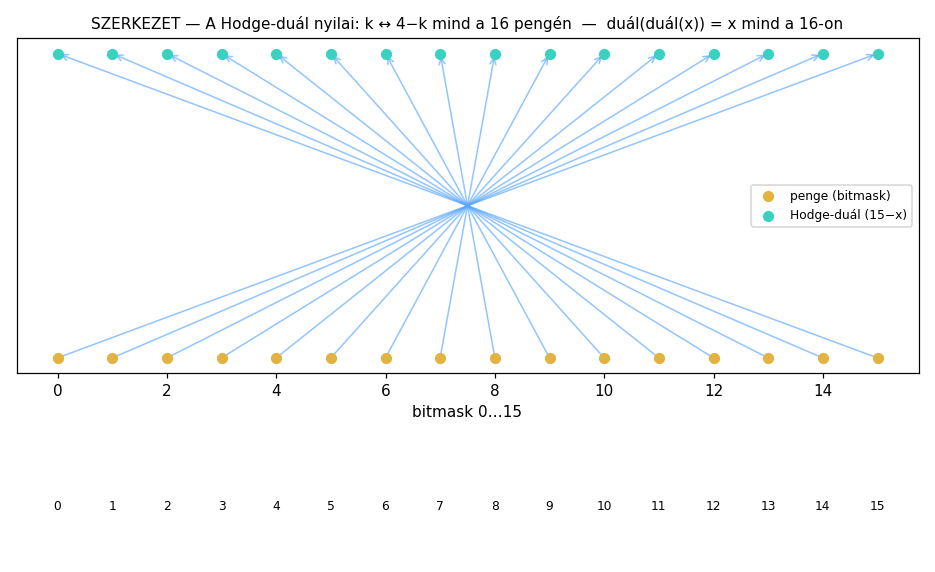
\includegraphics[width=0.42\textwidth]{docs/konyv/e8gyokrendszer/grafikonok/F2.29_1.png}
\end{center}
\nyelvPar{Balra az eloszlás (\texttt{F2.20}), jobbra a Hodge-duál a 16 pengén (\texttt{F2.29}): $\text{duál}(\text{duál}(x))=x$. Kapcsolódás: \href{https://en.wikipedia.org/wiki/Hodge_star_operator}{Hodge star operator}.}{\textit{Left: the distribution; right: the Hodge dual on the 16 blades: $\text{dual}(\text{dual}(x))=x$. See also: \href{https://en.wikipedia.org/wiki/Hodge_star_operator}{Hodge star}.}}

\subsection{E8 $\times$ E8 = 496 és a 248}\label{kartya:dimenzio}
\nyelvPar{Az $E_8$ dimenziója $240+8=248$ (gyökök + Cartan-algebra); a heterotikus húrelmélet mértékcsoportja $E_8\times E_8$ dimenziója $248\cdot2=496$. Mindkét szám \texttt{Refl}-lel rögzített (\texttt{bizE8E8Dimenzio}).}{\textit{The dimension of $E_8$ is $240+8=248$; the heterotic string gauge group $E_8\times E_8$ has dimension $496$. Both numbers are kernel-fixed.}}
\begin{center}
\begin{tikzcd}
240 \arrow[r, "+8"] & 248 \arrow[r, "\cdot\, 2"] & 496 \arrow[r, "="] & E_8\times E_8
\end{tikzcd}
\end{center}

\subsection{A 240 szó — híd a nyelv fejezetéhez}\label{kartya:nyelv}
\nyelvPar{A 240 gyök a Szima 3D-nyelvének alapszókincse (\texttt{GyökSzó}): 112 állandó fogalom + 128 kapcsolati fogalom; a jelentés a gyökök belső szorzattávolsága. A következő fejezet (F4) ezt a réteget építi tovább.}{\textit{The 240 roots are the basic vocabulary of the Szima 3D language (\texttt{GyökSzó}): 112 constant + 128 relational concepts; meaning is inner-product distance. The next chapter (F4) continues this layer.}}

\subsection*{A pilot futás GAUGE-táblája}
\begin{center}\small
\begin{tabular}{lrr}
\hline
név & szimuláció & kernel \\
\hline
típus-1 gyökök & 112 & 112 \\
típus-2 gyökök & 128 & 128 \\
E8 gyökök & 240 & 240 \\
$C(8,2)$ & 28 & 28 \\
$2^8$ & 256 & 256 \\
$8!$ (két út) & 40\,320 & 40\,320 \\
$W(D_8)=2^7\cdot 8!$ & 5\,160\,960 & 5\,160\,960 \\
trialitás & 135 & 135 \\
$W(E_8)$ & 696\,729\,600 & 696\,729\,600 \\
\hline
\end{tabular}
\end{center}
\nyelvPar{Forrás: \texttt{docs/konyv/e8gyokrendszer/main\_kimenet.txt} és \texttt{maradekok.csv} — minden sorban $\Delta=0$ (§1.0: Idris-generált Python; §18: két független út).}{\textit{Source: the pilot run files — every row $\Delta=0$ (Idris-written Python; two independent paths).}}

\end{document}
